\documentclass[11pt]{article}
\usepackage{minibox}
\usepackage[top=1in, bottom=1.25in, left=1.25in, right=1.25in]{geometry}
\newcommand{\tabitem}{~~\llap{\textbullet}~~}
\usepackage[parfill]{parskip}
\usepackage{enumerate}
\usepackage{amsmath}
\usepackage{amsthm}
\usepackage[shortlabels]{enumitem}
\usepackage{amssymb}
\usepackage{ bbold }
\usepackage{graphicx} %included to insert a graph
\usepackage{caption} %included to include a caption over the graph
\usepackage{booktabs} %needed for the table's toprule midrule and bottomrule sequences
\usepackage[section]{placeins} %to keep graphs and tables in the very section to which they belong 
\usepackage{pdflscape} %to include the landscape environment 
\usepackage[T1]{fontenc}
\usepackage{multirow}
\usepackage{verbatim}
\usepackage{subcaption}
\usepackage{pdfpages}
\usepackage{lscape}
%-----------------------------------------------------------------------------
\begin{document}
\begin{center}
\framebox[\linewidth]{ 
	\minibox[c]{
	\Large Econ 244 - Homework \#4 \\ \\
	}
}
\end{center}

\begin{enumerate}[(a)]
	\item See do file.
	\item See do file and table \ref{q2b}. \\
	\begin{table}[htbp]\centering \scriptsize
\def\sym#1{\ifmmode^{#1}\else\(^{#1}\)\fi}
\caption{Question 2b and 2e \label{q2b}}
\begin{tabular}{l*{2}{c}}
\toprule
                    &\multicolumn{1}{c}{(1)}&\multicolumn{1}{c}{(2)}\\
                    &\multicolumn{1}{c}{Log Arrests}&\multicolumn{1}{c}{Log Arrests}\\
\midrule
0                   &     -0.0724*  &     -0.0447   \\
                    &   (0.04097)   &   (0.03410)   \\
\addlinespace
1                   &      -0.153** &     -0.0994*  \\
                    &   (0.06718)   &   (0.05405)   \\
\addlinespace
2                   &      -0.179*  &      -0.103   \\
                    &   (0.09928)   &   (0.08530)   \\
\addlinespace
3                   &      -0.196*  &     -0.0969   \\
                    &   (0.11195)   &   (0.09814)   \\
\addlinespace
4                   &      -0.216   &     -0.0984   \\
                    &   (0.13955)   &   (0.13022)   \\
\addlinespace
5                   &      -0.254   &      -0.127   \\
                    &   (0.15976)   &   (0.15272)   \\
\addlinespace
6                   &      -0.337*  &      -0.188   \\
                    &   (0.18844)   &   (0.18051)   \\
\addlinespace
7                   &      -0.381*  &      -0.225   \\
                    &   (0.21022)   &   (0.21005)   \\
\addlinespace
8                   &      -0.357*  &      -0.206   \\
                    &   (0.21014)   &   (0.21727)   \\
\addlinespace
9                   &      -0.463*  &      -0.293   \\
                    &   (0.25040)   &   (0.25997)   \\
\addlinespace
10                  &      -0.561*  &      -0.423   \\
                    &   (0.31938)   &   (0.37817)   \\
\addlinespace
-2                  &     0.00306   &     -0.0266   \\
                    &   (0.04029)   &   (0.03919)   \\
\addlinespace
-3                  &      0.0505   &     -0.0118   \\
                    &   (0.06806)   &   (0.06462)   \\
\addlinespace
-4                  &      0.0744   &     -0.0217   \\
                    &   (0.09482)   &   (0.07838)   \\
\addlinespace
-5                  &      0.0634   &     -0.0682   \\
                    &   (0.12321)   &   (0.09156)   \\
\addlinespace
-6                  &      0.0756   &      -0.116   \\
                    &   (0.15743)   &   (0.11055)   \\
\addlinespace
-7                  &      0.0681   &      -0.163   \\
                    &   (0.19197)   &   (0.13063)   \\
\addlinespace
-8                  &      0.0822   &      -0.174   \\
                    &   (0.22642)   &   (0.15078)   \\
\addlinespace
-9                  &      0.0243   &      -0.277   \\
                    &   (0.26328)   &   (0.17508)   \\
\addlinespace
-10                 &      0.0862   &      -0.342   \\
                    &   (0.33427)   &   (0.20880)   \\
\addlinespace
Constant            &       6.545***&       6.556***\\
                    &   (0.26179)   &   (0.10881)   \\
\midrule
Year Fixed Effects & X & X \\
City Fixed Effects & X & X \\
City-Specific Time Trend & & X \\
\midrule
\(R^{2}\)           &       0.804   &       0.870   \\
Observations        &        1297   &        1297   \\
\bottomrule
\multicolumn{3}{l}{\footnotesize Standard errors in parentheses}\\
\multicolumn{3}{l}{\footnotesize * p<0.10, ** p<0.05, *** p<0.01}\\
\end{tabular}
\end{table}

	\item  It appears arrests go down in the years following the policy relative just before the curfew was put in place. In the years prior to the policy, arrest rates were fairly flat. However, the estimates are fairly imprecise outside of a couple year band around the policy. Note that data from 10 years before the policy and 10 years after were binned into the -10 and 10 dummies.\\
	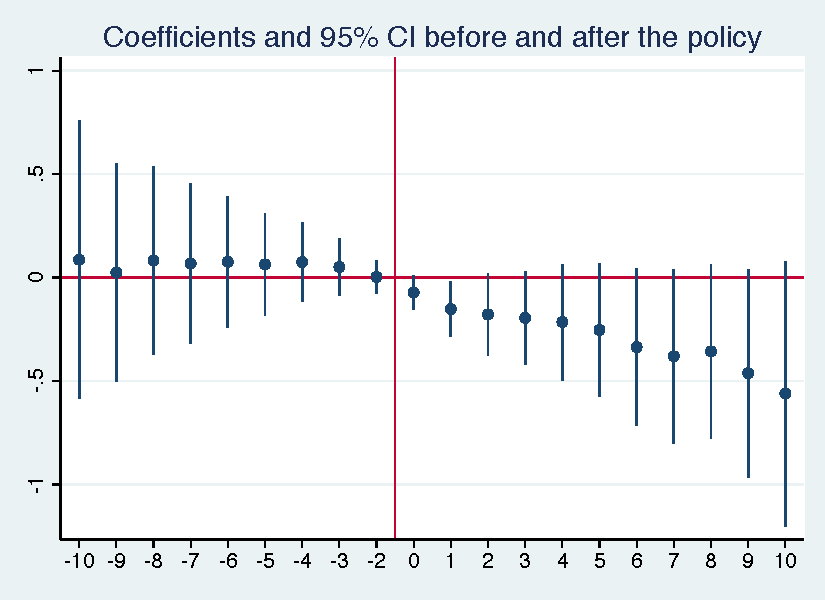
\includegraphics[scale=.8]{input/coef_plot_10year.pdf}
	\item We can restrict our analysis to just look 5 years before and after the policy or 12 years before and after. We can see a slight change in the coefficients but the general pattern is similar--that arrest rates were fairly flat beforehand and decreased in the years after the policy.\\
		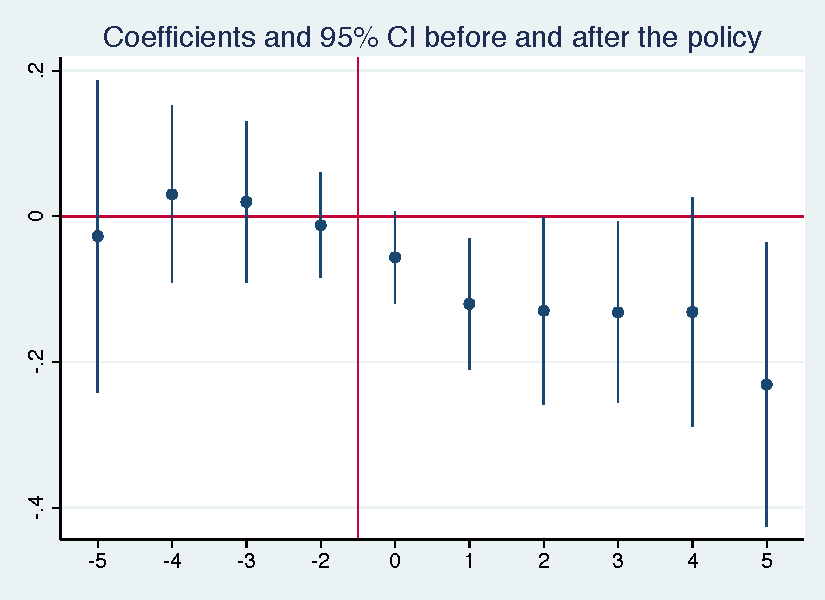
\includegraphics[scale=.8]{input/coef_plot_5year.pdf} \\
		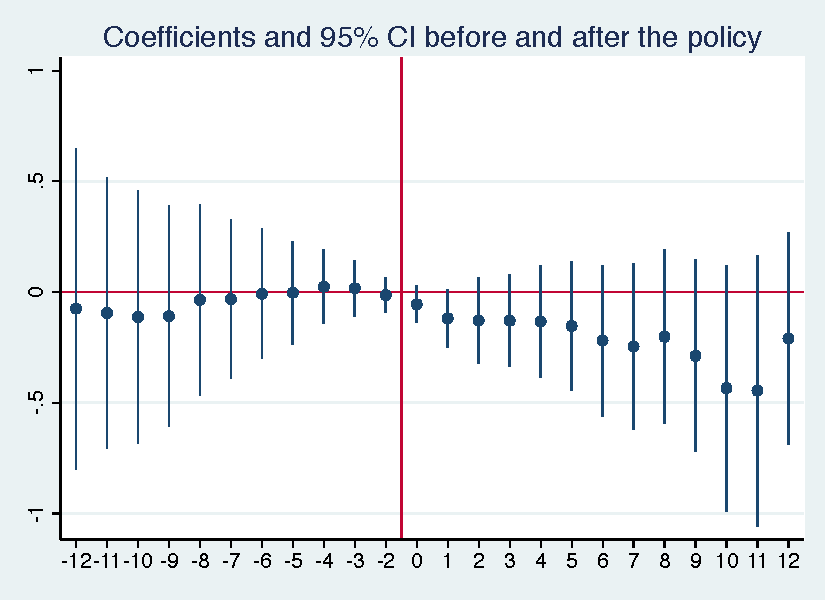
\includegraphics[scale=.8]{input/coef_plot_12year.pdf}
	
	\item When we add a linear city-specific trend, we get a slightly different story from the data. It appears that arrests were slightly increasing prior to the policy change and then decreased afterwards. Perhaps explaining the impetus for the policy change. \\
		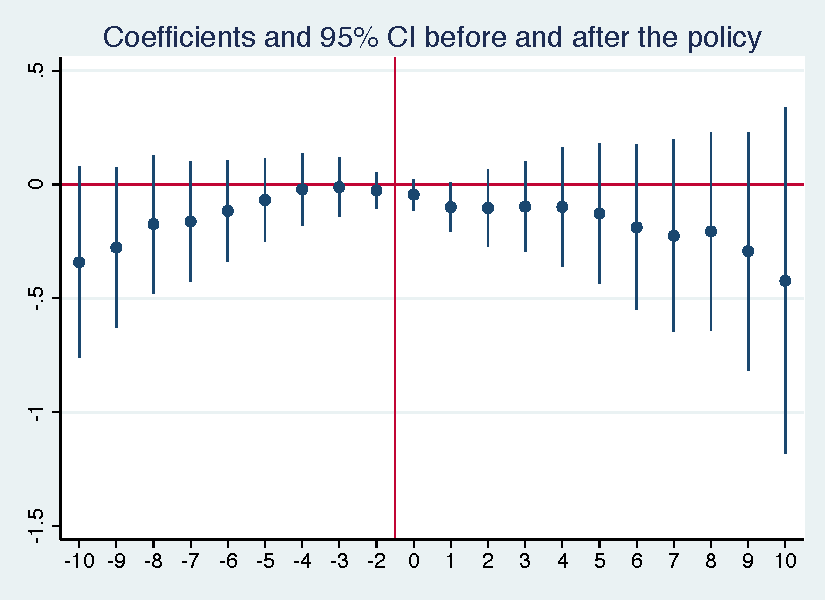
\includegraphics[scale=.8]{input/coef_plot_10year_trend.pdf}
	
\end{enumerate}


\end{document}